\documentclass[9pt]{article}

\usepackage{graphicx}
\usepackage{graphics}
\usepackage[normalsize]{subfigure}

\title{Programming Assignment Part III}
\author{
    Kelly Kaoudis \\
    CSCI 6564, Fall 2013 \\
}
\date{\today}

\begin{document}
\maketitle

\section{Deliverable}
\begin{enumerate}
    \item implement and compare two or more entering variable
    selection strategies: Bland's rule and the max coefficient
    rule
    \item measure effect of entering variable strategy on runtime
    \item use cubic least squares to explain, for both, the runtime
    as a function of the problem size, visually
\end{enumerate}

\section{Implementation and discussion}
Starting with my code from step two, which functions well for m $<=$ n,
I built a framework to test my entering rules against each other. Then I
took what I had for the default solver implementation from the second
step, which uses the largest coefficient rule, and replaced LC with Bland.

A difference between the two rules' results was in the case of unbounded
problems; perhaps it's a bug in my implementation, but sometimes
when the largest-coefficient
solver sees an unbounded problem, the Bland's solver seems
to be able to find an optimal solution. Other than that, the two rules consistently get the same optimal value even for a few of the evil problems.

\begin{table}[ht]
\centering
\begin{small}
\begin{tabular}{l l l l l l}
    Rule & problem size & steps & $\zeta$ & stalls & time \\ [0.5ex]
    \hline
    largest coef. & 10 by 10 & 4 & .066223 & 0 & 0.000956 sec \\
    Bland's & 10 by 10 & 6 & .066223 & 0 & .0013 sec \\
    largest coef. &  15 by 15 & 4 & .264389 & 0 & .0011 sec \\
    Bland's & 15 by 15 & 7 & .264389 & 0 & .0014 sec \\
    largest coef. & 20 by 20 & 5 & unbounded & 0 & .0012 sec \\
    Bland's & 20 by 20 & 8 & unbounded & 0 & .0014 sec \\
\end{tabular}
\caption{Revised simplex over randomly generated sparse problem instances using two entering variable selection rules.}
\end{small}
\end{table}

\begin{table}[ht]
    \centering
    \begin{small}
    \begin{tabular}{l l l l l l}
        Rule & problem size & steps & $\zeta$ & stalls & time \\ [0.5ex]
        \hline
        largest coef. & 10 by 10 & 6 & unbounded & 0 & .0026 sec \\
        Bland's & 10 by 10 & 9 & unbounded & 0 & .0027 sec \\
        largest coef. & 15 by 15 & 11 & 3.37889 & 0 & .0024 sec \\
        Bland's & 15 by 15 & 20 & 3.37889 & 0 & .0038 sec \\
        largest coef. & 20 by 20 & 12 & 1.489563 & 0 & .0028 sec \\
        Bland's & 20 by 20 & 50 & 1.489563 & 0 & .0107 sec \\
        largest coef. & 50 by 50 & 72 & 4.133696 & 0 & .0250 sec \\
        Bland's & 50 by 50 & 325 & 4.133696 & 0 & .1031 sec \\
    \end{tabular}
\caption{Revised simplex over randomly generated dense problem instances.}
\end{small}
\end{table}

\begin{small}
\begin{figure}[tbp]
\centering
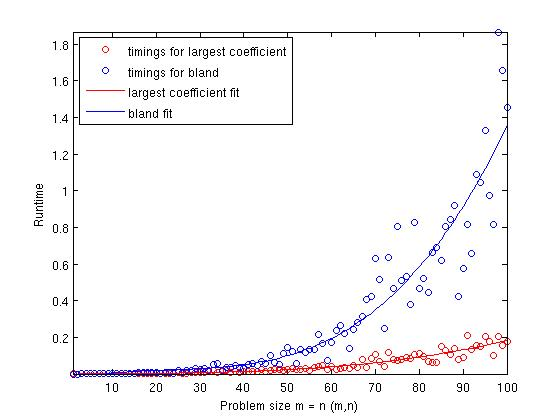
\includegraphics[scale=0.5]{m100blandversuslc.jpg}
\caption{An illustration of Bland's rule versus the largest coefficient rule on
a hundred randomly generated dense problem instances with m, n equal and ranging from 1 to
100. The two curves are cubic least-squares approximations to the data, coloured respectively.}
\end{figure}

\begin{figure}[tbp]
\centering
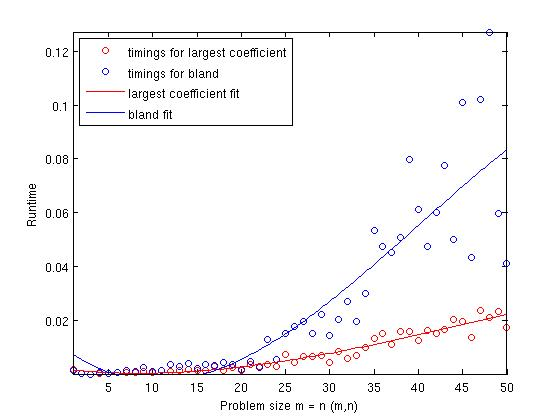
\includegraphics[scale=0.5]{m50blandversuslc.jpg}
\caption{A closer look at Bland's versus largest coefficient for m = n = 1:50 on randomly generated dense
problem instances, again fitted using a cubic least squares regression model.}
\end{figure}

\begin{figure}[tbp]
\centering
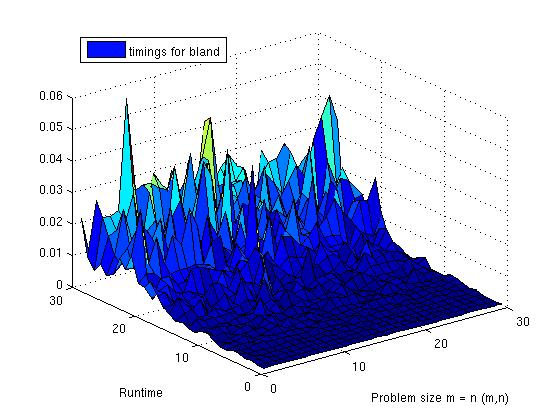
\includegraphics[scale=0.5]{m30blandtimingversussize.jpg}
\caption{Solver runtime versus problem size where m = n for Bland's rule on dense problem instances between 1 and 30.}
\end{figure}

\begin{figure}[tbp]
\centering
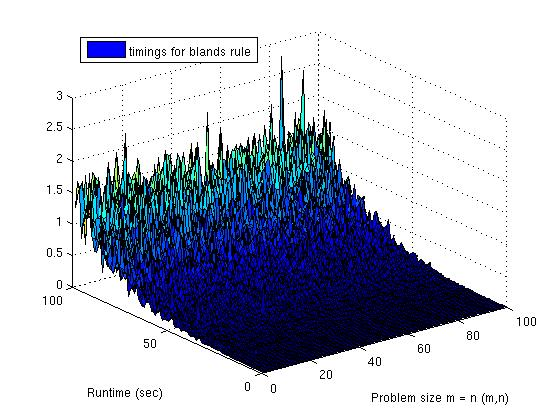
\includegraphics[scale=0.5]{m100blandtimingversussize.jpg}
\caption{Solver runtime versus problem size where m = n for Bland's rule on dense problem instances between m = n = 1 to 100.}
\end{figure}

\begin{figure}[tbp]
\centering
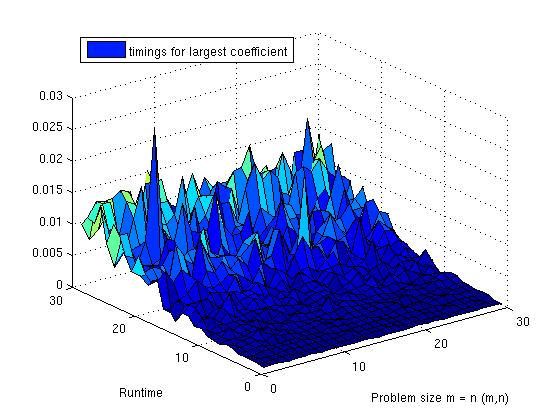
\includegraphics[scale=0.5]{m30lctimingversussize.jpg}
\caption{Solver runtime versus problem size, m = n, for the largest coefficient rule on dense problem instances for m = n = 1 to 30. Comparing this plane to the one generated from Bland's for time versus size, it appears that the ditribution in this case is somewhat more uniform.}
\end{figure}

\begin{figure}[tbp]
\centering
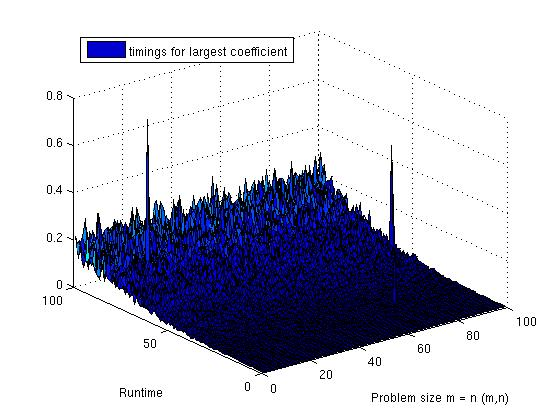
\includegraphics[scale=0.5]{m100lctimingversussize.jpg}
\caption{Solver runtime versus problem size for m = n = 1 to 100 for the largest coefficient rule. Barring two spikes for what the solver reported as problem instances with multiple stalls, this distribution also appears more even than the comparable Bland's version.}
\end{figure}
\end{small}
\section{Results and conclusions}
Bland's rule consistently takes longer
because it usually performs more steps than the largest
coefficient rule across dense and sparse cases of varying
sizes in revised simplex. Generally, as problem density
increases across size, the solver takes longer using
either rule. The time the solver takes to run
increases with problem size for dense and sparse varieties of matrix.
While I would have liked to look at more sparse instances
and at the steepest-edge and greedy rules,
I'll save that for later exploration.

\end{document}
